\documentclass[letterpaper,12pt]{article}

\usepackage{mathpazo}
\usepackage[longnamesfirst]{natbib}
\usepackage[flushleft]{threeparttable} 
\usepackage{booktabs}
\usepackage{rotating} 
\usepackage{amssymb} 
\usepackage{amsmath}
\usepackage{caption} 
\usepackage{dcolumn} 
\usepackage{setspace}
\usepackage[longnamesfirst]{natbib}
\usepackage[font=scriptsize]{subfig}
\usepackage[pdftex,colorlinks=true,linkcolor=black,citecolor=black]{hyperref} 
\usepackage[margin=1.0in]{geometry} 
\usepackage{multirow}

\newcommand{\mco}[1]{\multicolumn{1}{c}{#1}}
\newcommand{\mct}[1]{\multicolumn{2}{c}{#1}}


%opening
\title{Fertility Issues in Developing Countries} 

\author{Claus C P\"ortner\\
    Department of Economics\\
    Albers School of Business and Economics\\
    Seattle University, P.O. Box 222000\\
    Seattle, WA 98122\\
    \href{mailto:cportner@seattleu.edu}{\texttt{cportner@seattleu.edu}}\\
    \href{http://www.clausportner.com}{\texttt{www.clausportner.com}}\\
    \& \\
    Center for Studies in Demography and Ecology \\
    University of Washington\\ \vspace{2cm}
    }

\date{February 2017}

\doublespacing

\begin{document}
\graphicspath{{../figures/}}
\DeclareGraphicsExtensions{.jpg,.jpeg,.pdf,.mps,.png}

\maketitle
\thispagestyle{empty}


\newpage

\section{Introduction}

Despite a common perception that fertility is very high in developing countries,
the truth is substantially more complicated.
Figure \ref{fig:TFR} shows that there has been an astonishing decline in total 
fertility rate (TFR) in developing countries over the last half century.%
\footnote{
TFR is the number of children a women entering her reproductive life
would have if she had children following the age-specific fertility
rates observed at that point in time.
Hence, it is composite or snapshot measure of current fertility
behavior.
}
Half a decade ago, TFR was around 7 children, with the exception
of TK.
The most recent data show, however, that, with the exception of 
Sub-Saharan African, TFR is now either below or only slightly 
above the replacement level of 2.1.
Despite this rapid decline in fertility population size is still
growing in many of these regions because there are still many
more young people than older people and these young people either
have not entered reproductive age or are just starting out.

\begin{figure}[hp]
    \centering
    \caption{Total Fertility Rates by Region from 1967 to 2015}
    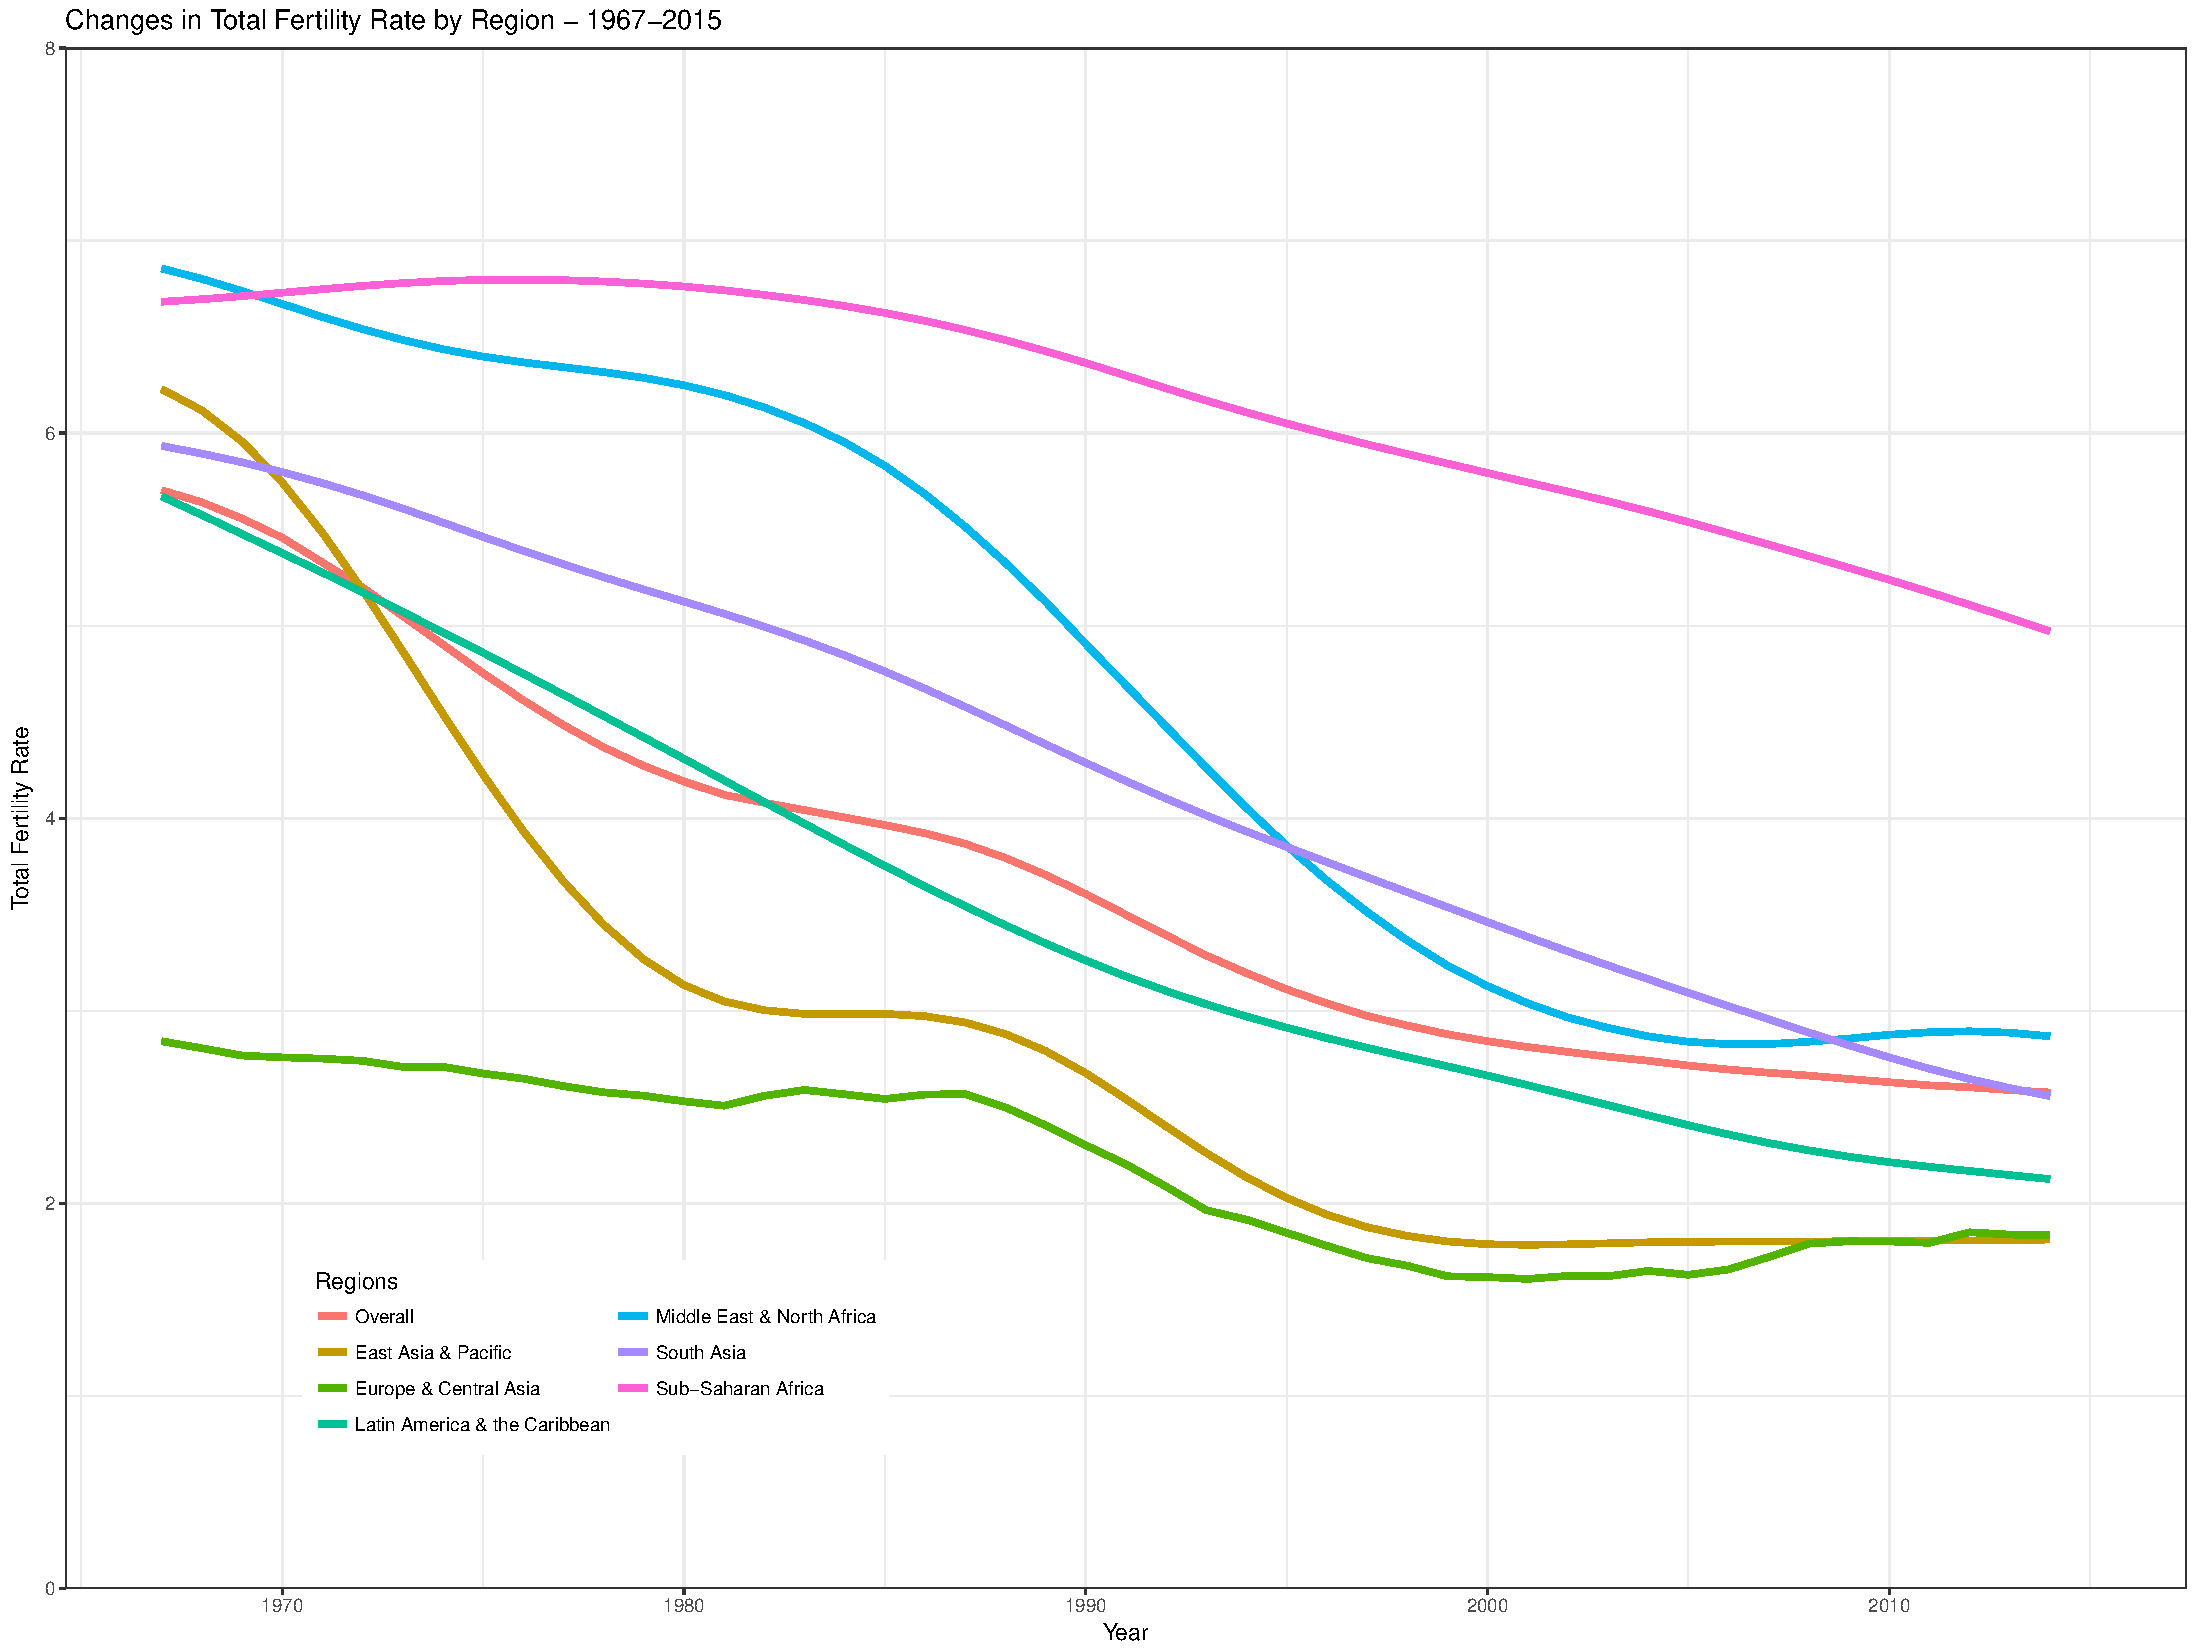
\includegraphics[width=0.75\linewidth]{totalFertilityRates}
    \label{fig:TFR}
\end{figure}

If fertility levels are close to identical across developing and
developed countries and there is rapid urbanization and increasing
labor force participation among women do we even need a developing 
country version of this chapter?%
\footnote{
TK references on urbanization and labor force particpation.
}
The goal of this chapter is to highlight the areas in which a
separate focus on developing countries is still relevant,
what the recent developments in research has been, and
most importantly, what I consider to be the main
outstanding issues.

[still need policy discussion; this seems kind of a rambling list]
Furthermore, we still know relatively little about determinants
of timing of births in developing countries.
People in most developing countries are also still subject to
higher risk of shocks, be that from weather, health, or political,
but we still have little idea of how people respond to the level
of risk and the occurrence of shocks.
Finally, both in developed and developing countries we have
mostly treated fertility decisions as separate from other
household decision and preferences [ehh, Becker theory!].
We still need to know more about how husband and wife decides
on fertility if they are have different preferences 
and how allocation decisions across all household member are
related to fertility decisions.
A prime example that I will treat separately is the role
of son preferences in fertility decisions.









\section{Sub-Saharan Africa}

[\citet{Ainsworth1996a} introduction to a symposium on fertilit
in Sub-Saharan Africa]

The outlier in the figure above is Sub-Saharan Africa. 
Sub-Saharan Africa now has an average TFR that is about twice
as large as the other regions.
Most of the projected future increase in world population 
is therefore likely to come from Sub-Saharan Africa 
\citep{Gerland2014}.%
\footnote{
Currently Africa is home to about 1 billion people, but this
will increase to between 3.1 and 5.7 billion by the end of
the century.
}
The most important issues from a policy standpoint is why the 
fertility decline in Sub-Saharan Africa have moved at a much
slower pace than the other regions.
The purpose of this is not to provide the final answer, but
instead to highlight both how we can think about fertility
decisions and suggest possible answers.

Broadly speaking there are two competing approaches to 
explaining fertility decisions.%
\footnote{
This is clearly a simplification but it serves to illustrate
the differences in approaches.
}
One sees fertility preferences as the main driver of fertility and
considers preferences malleable and mainly determined by cultural 
factors and transmission of ideas of ideal family size across groups.
Under this approach the main constraints on reaching desired 
fertility is the level of access to family planning and 
contraceptives.

The other sees the decision on fertility as driven by the
trade-off between the cost of children and the return to children,
which can either be monetary or the utility of having offspring.
In this approach parents are assumed to be able to control 
fertility even in the absence of modern contraceptives.
Hence, although lower cost of preventing births---for example
easier access to modern contreceptive---will still lower
fertility in this approach the decline in fertility is 
assumed to be much smaller than the first theory.

Both theories consider the surviving number of children as
the main outcome that people are interested in.
One possible explanation for the slow decline in fertility
could therefore be that mortality in Sub-Saharan Africa is
higher than in the other regions.
Figure \ref{fig:mortality} shows the development over time in 
under-5 mortality across the same regions as above.
The improvements in mortality risk over time are truly astonishing.
Over the last half-decade under-5 mortality in developing countries 
has fallen from close to 175 to below 50 per 1,000 live births.
Sub-Saharan Africa, however, lacks substantially behind other regions.
Despite a massive improvement from a situation where more than a
quarter of all children born did not live to see their fifth
birthday to about 80 deaths per 1,000 births, the current mortality 
rate is still more than three times larger than that of the other 
regions (with the exception of Middle East and North Africa).
Although mortality is likely part of the explanation it cannot
be the full explanation.
Mortality in Sub-Saharan Africa is at the same level as it was
in South Asia around the turn of the century, but fertility
is about 1.5 child higher in Sub-Saharan Africa than it was
in South Asia at the turn of the century (and therefore at the
same level of mortality).

\begin{figure}[hp]
    \centering
    \caption{Under-5 Mortality Rates by Region from 1967 to 2015}
    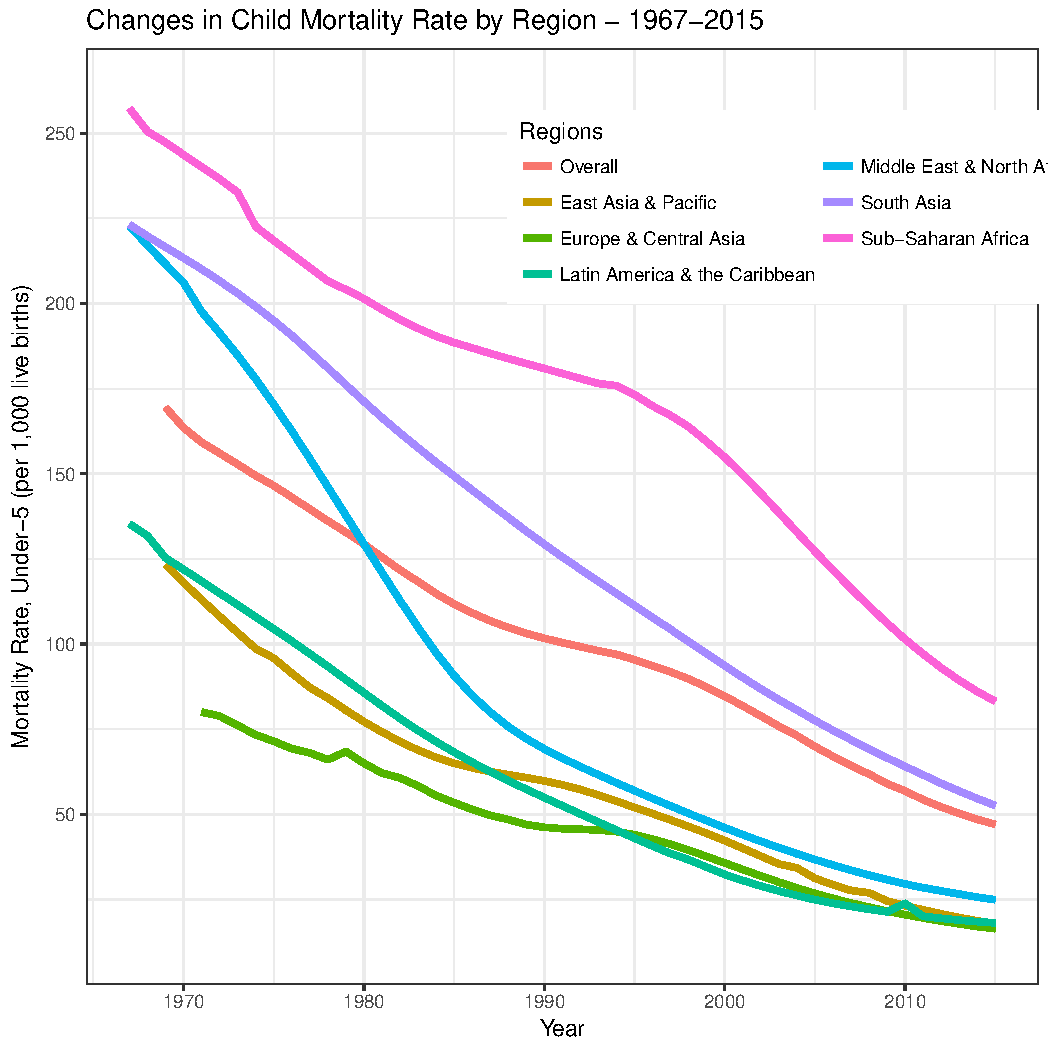
\includegraphics[width=0.75\linewidth]{childMortalityRates}
    \label{fig:mortality}
\end{figure}

If mortality is not the explanation, what might lead to the
higher fertility in Sub-Saharan Africa?
Demographers, following the first approach described above, 
have argued that the two main reasons for the slow decline 
in fertility in Sub-Saharan Africa are the high ideal family 
size still in place and a substantial ``unmet need'' for contraception  
\citep{Bongaarts2013a}.
Contraceptive use is, indeed, lower in Sub-Saharan Africa than
the other regions, but other regions managed to reduced fertility
even in the absence of access to modern contraceptives 
[TK add reference on Europe].
Furthermore, one difference in fertility behavior between 
Sub-Saharan Africa and the other regions are that the longer 
birth intervals even in the absence of access to modern 
contraception, which are the result of postpartum sexual 
abstinence and extended periods of breastfeeding \citep{Caldwell1992}.
To the extend that the longer birth intervals are the result
of conscious decisions it shows that people are able to
control fertility.%
\footnote{
It is still possible that fertility is higher than desired
because the higher cost of preventing ``accidental''
conceptions.
This would explain why the estimated effect of access to 
family planning in Ethiopia shows a reduction in fertility
of about one birth, which is equivalent to an approximate
20\% reduction in fertility \citet{Portner2014a}.
}


There are three alternative explanation that may explain the
slow decline.
First, the relative abundance of land compared to other regions.
Second, low levels of education; or at least low levels of quality
in education.
Finally, differences in urbanization across regions.  

[Land - see Caldwell1992, higher return to children,
also mention the issues with land rights \citep{Goldstein2008}
and high return to women on agricultural land \citep{jacoby95}]

land pressure low even at the high projected  population growth
See Gerland2014

[Education data; might be less reliable in terms of actual
human capital accumulation; see Tanzania for an example]


\citet{Marchetta2016} argues that the literature shows that
fertility only declines at higher levels of education in
Sub-Saharan Africa. See  \citet{Ainsworth1996}, \citet{Thomas1996}


[urbanization; urban vs rural - Ethiopia as an example]




    

\section{Timing of Fertility}

As the figure above shows 


\citet{Dupas2017}

\citet{Marchetta2016}

\citet{Duflo2015}

\section{Intrahousehold Allocation}



\citet{Ashraf2014}

\cite{merli00} on missing girls in China



\section{Policies}


Schultz paper on Matlab and improvements in women's lives.

Disruption in access: \citet{Dumas2017}

\section{Conclusion}


\bibliographystyle{aer}
\bibliography{collection}


\end{document}
